\section{Implementing the User Interface}\label{sec:impinterface}
As stated in \cref{sec:serverInterface} the usability of the server interface was not consideret. Therefore this section focus on explaining how previously explained functionality is implemented and can be achieved by the administrator.

The first screen the administrator meets when opening the application is the login screen for spotify, as seen in \cref{fig:loginInterface}. Here the administrator inputs the login credentials for the venues Business Spotify Account (see \cref{ch:preface} for legal terms). This is used to get the data needed to play songs from spotify's catalogue. From this interface the administrators and stop and start the playback of music as described in \cref{systemDefinition}. Also the icon for the application acts as a skip button where administrators can skip the currently playing track.

\begin{figure}[H]\label{fig:loginInterface}
  \centering
  \subfloat{
    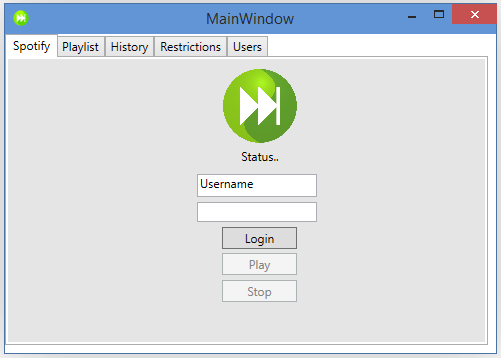
\includegraphics[width=0.5\textwidth]{ServerInterfaceLogin}
  }
  \subfloat{
    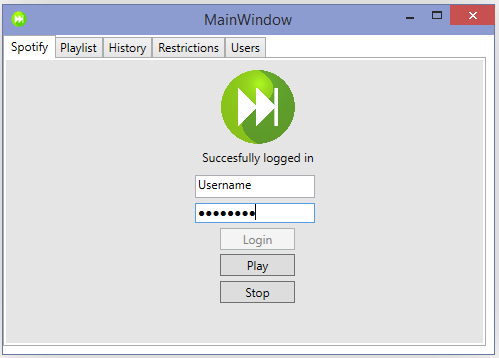
\includegraphics[width=0.5\textwidth]{ServerInterfaceLoggedin}
  }
  \caption{Login interface on the server.}
\end{figure}

The second interface is the playlist and can be seen in \cref{fig:ServerInterfacePlaylist}. Here the most crucial information about tracks on the playlist can be seen; the title, artist(s), duration (in milliseconds), temporary and permanent votes. The album cover is also displayed for the ability to quickly identify tracks. The playlist is ordered in the order they will be played, the higher a placement, the sooner it will be played. From this interface further administrative control can be executed including removal of specific tracks and rearrangement of the playlist as described in \cref{systemDefinition}. When pressing the move up or move down button the currently selected track changes one position, this is done through changing the permanent votes just enough for the track to change place.

\begin{figure}[hbtp]
  \centering
  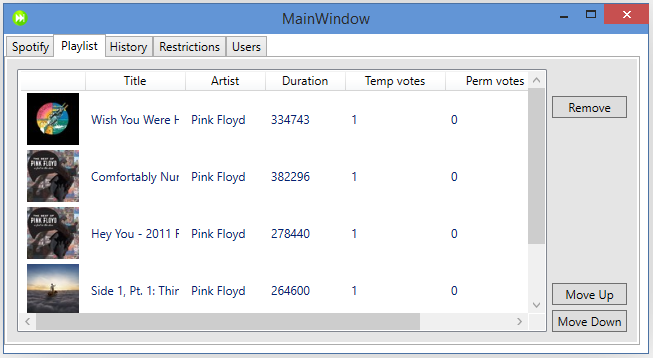
\includegraphics[width=\textwidth]{Images/ServerInterfacePlaylist.png}
  \caption{Playlist interface on the server.}\label{fig:ServerInterfacePlaylist}
\end{figure}

The third interface is the history interface, seen in \cref{fig:ServerInterfaceHistory}. From here the administrator can see what was been played previously. The higher on the list the longer ago it has been played. Like the playlist interface only the most crucial information is displayed, therefore all votes are removed since these are not important any longer.

\begin{figure}[hbtp]
  \centering
  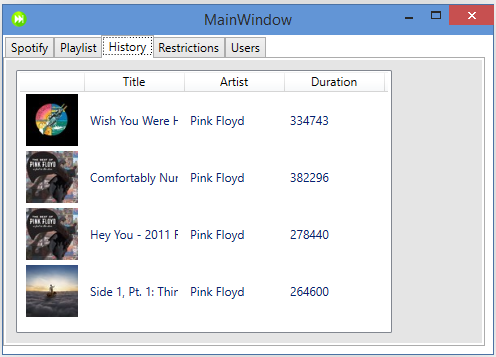
\includegraphics[width=\textwidth]{Images/ServerInterfaceHistory.png}
  \caption{History interface on the server.}\label{fig:ServerInterfaceHistory}
\end{figure}

The fourth interface is the restriction interface and can be seen in \cref{fig:ServerInterfaceRestrictions1}. from here the administrator can modify, remove and add restrictions. Adding or modifying a restriction brings up a dialogue where parameters for the restriction according to \cref{sec:restrictions}.

\begin{figure}[H]
  \centering
  \subfloat[Main restriction interface.]{
    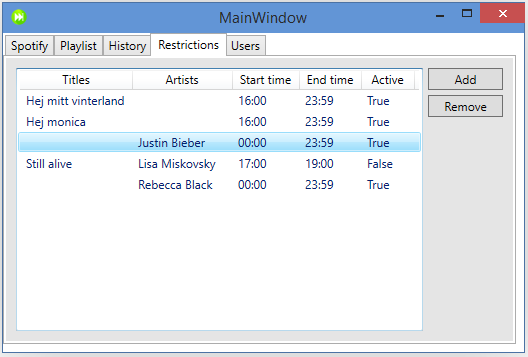
\includegraphics[height=160px]{ServerInterfaceRestrictions}
        \label{fig:ServerInterfaceRestrictions1}
  }
  \subfloat[Restriction modify dialogue.]{
    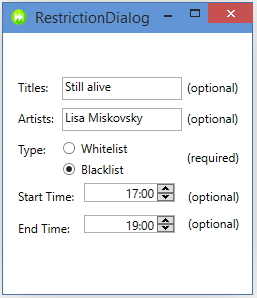
\includegraphics[height=160px]{ServerInterfaceRestrictionDialog}
        \label{fig:ServerInterfaceRestrictions2}
  }
  \caption{Restriction interface on the server.}
\end{figure}

The last interface is the user interface and can be seen in \cref{fig:ServerInterfaceUsers}. From here the administrator can keep track of how many and which guests have checked in at the venue. The administrator can see what they have voted, both an track and volume. The guests should here be represented via their unique ID as will be described in \cref{sec:UAuth}
\begin{figure}[hbtp]
  \centering
  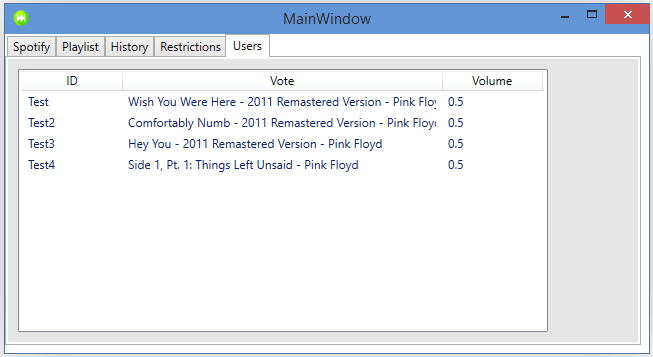
\includegraphics[width=\textwidth]{Images/ServerInterfaceUsers.png}
  \caption{User interface on the server.}\label{fig:ServerInterfaceUsers}
\end{figure}
